\begin{frame}{Research Proposal}
	\begin{center}
		\textbf{Acceleration of non-rigid image registration with Tensor Cores}
	\end{center}
	\begin{columns}
		\column{0.55\textwidth}
		\begin{itemize}
			\item Image registration: aligning 2 images
			\item \emph{Non-rigid}: various deformations allowed
			\item Use next-gen GPUs for acceleration
			\item \textbf{Goal: get closer to real-time (currently: seconds) for surgery} 
		\end{itemize}

		\column{0.45\textwidth}
		\begin{figure}
			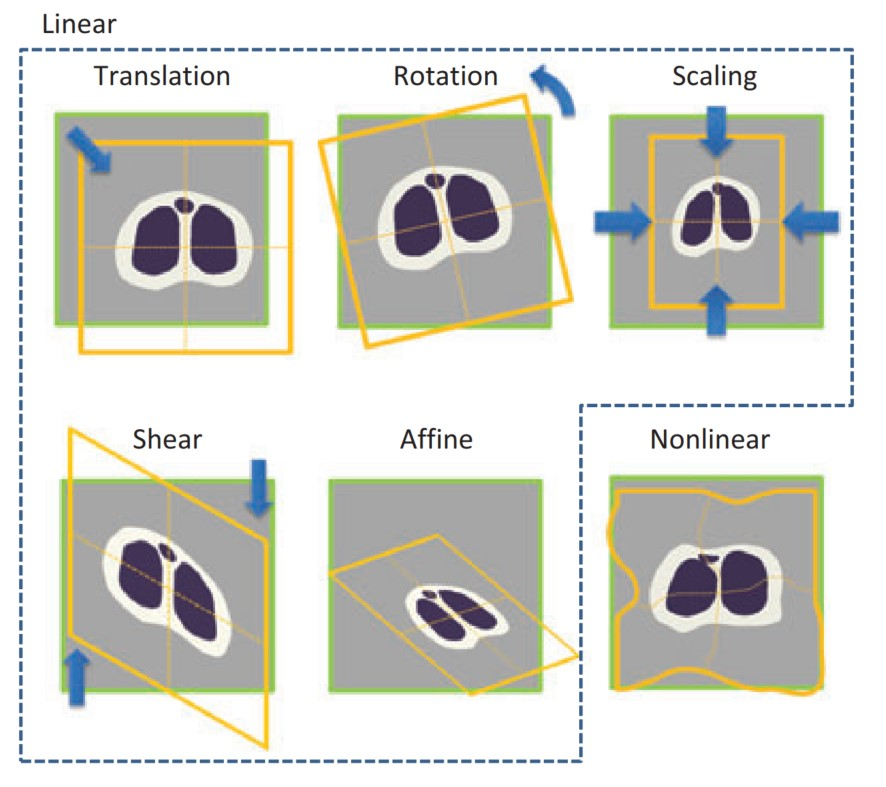
\includegraphics[width=\textwidth]{registration}
			\caption[Deformations]{Different types of deformation.}
			\label{fig:registration}	
		\end{figure}

	\end{columns}
	
\end{frame}